\section{Access model}

\noindent Since the SAT-attacker needs access to every flip-flop in the IC, this can be achieved by operating the IC in scan mode of operation by asserting the test mode signal. In today's SoCs, it is only possible to access the scan architecture through embedded deterministic test (EDT) architecture, the on-chip decompression/compression scheme, which also comes with a bypass mode for debug purposes. Moreover, the SAT-attacker wants to apply very specific values to these flip-flops to force the logic nodes to specific states and capture the exact responses, in order to decrypt one of the correct keys. This is possible only in the EDT-Bypass mode. In summary, the access model is (i) initializing flip-flops during scan shift; and (ii) using EDT bypass mode to have direct access to scan-chains. 

\begin{figure}
\centering
\includegraphics[scale=0.14]{fig/encrypted-DFT.pdf}
\caption{DFT Encryption}
\label{fig:encrypted-DFT}
\end{figure}


\begin{figure}
\centering
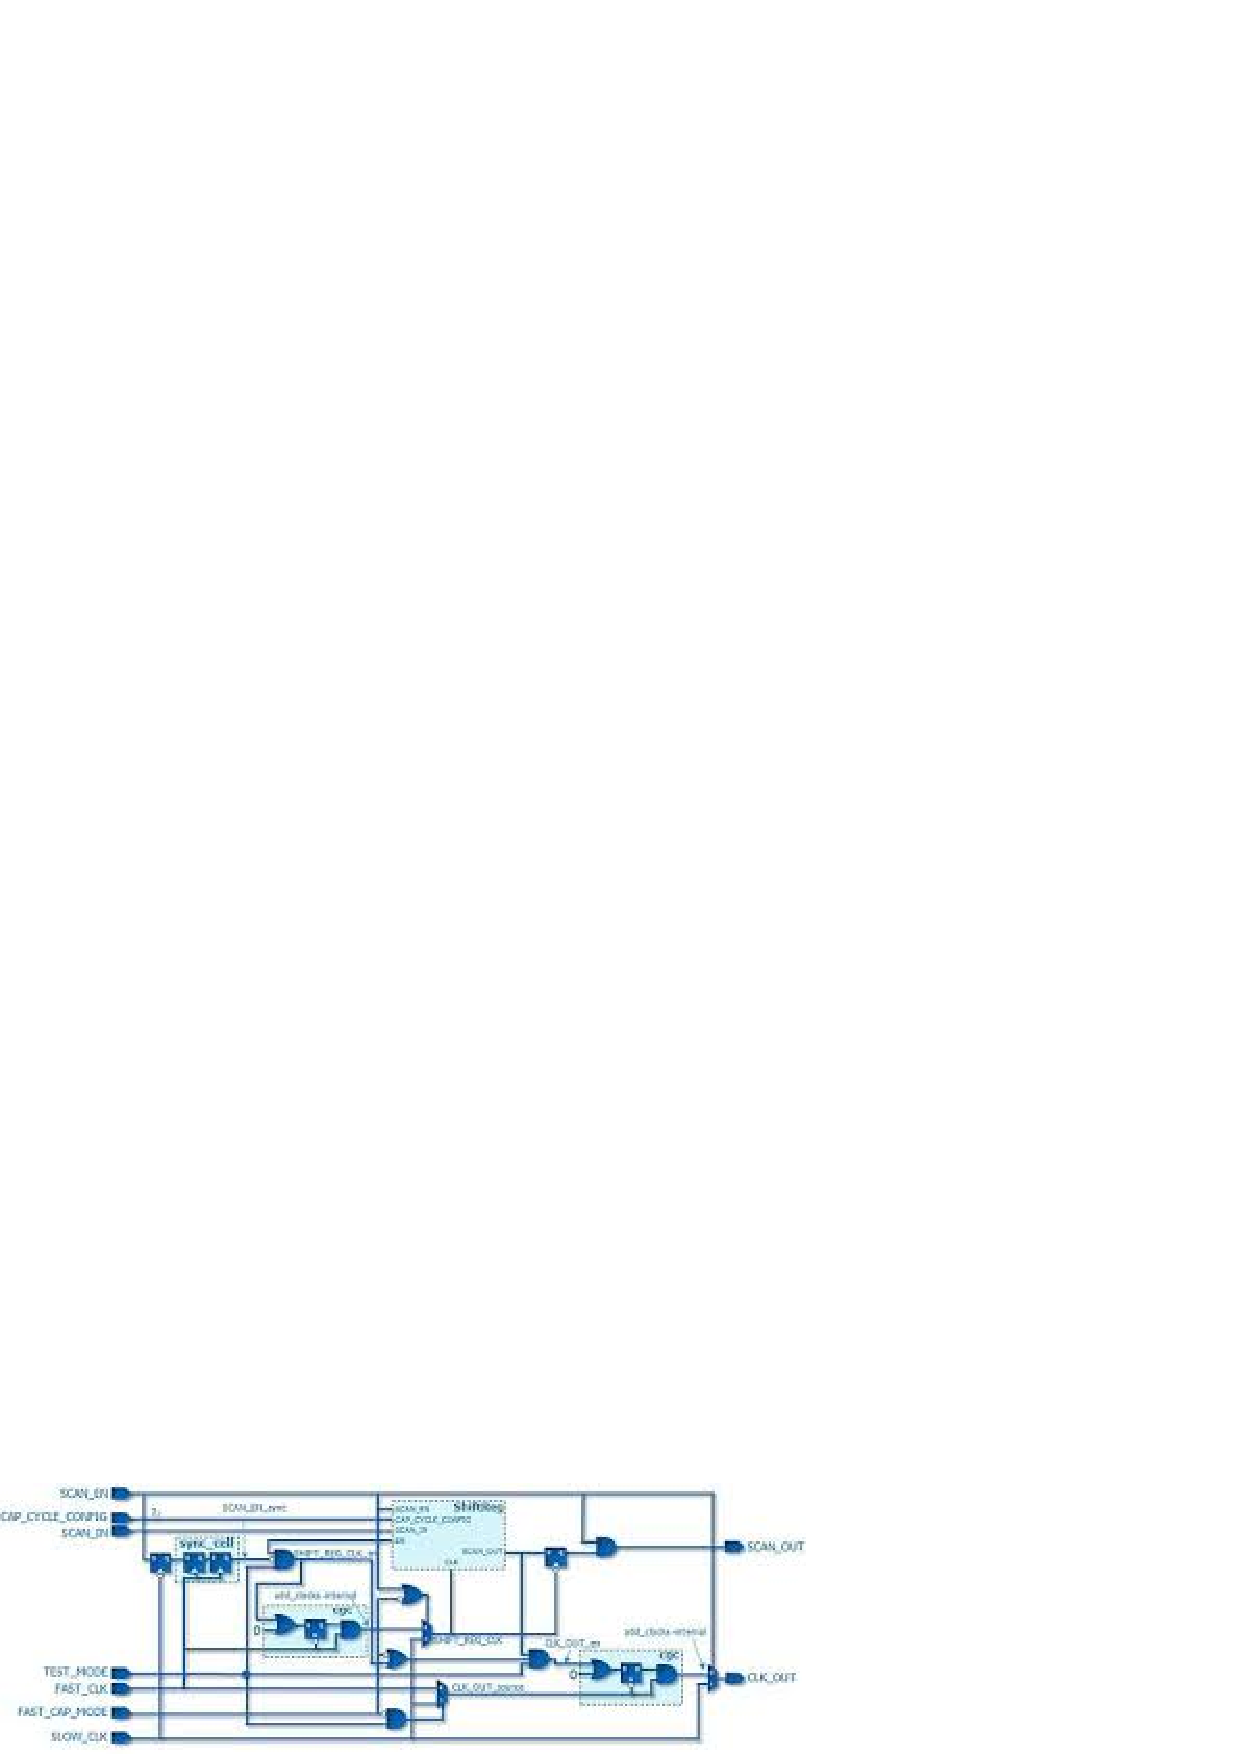
\includegraphics[scale=0.6]{fig/occ.pdf}
\caption{On-chip clock control}
\label{fig:occ}
\end{figure}


Figure~\ref{fig:encrypted-DFT} shows the encrypted design-for-testability (DFT) architecture, where both the combinational logic and flip-flops are encrypted, while the decompressor/compactor are unencrypted. 
Hence, the decompressor and compactor should be bypassed, to directly access the scan chains. Figure~\ref{fig:occ} shows the on-chip clock control scheme used in modern SoCs. The attacker places the IC in scan mode of operation by asserting $TEST\_MODE$ signal shown in this figure. To apply the desired input vector to the combinational portion of the IC, the attacker assigns the flip-flops to desired values by placing the IC in scan-shift mode, by further asserting $SCAN\_EN$ signal. After initialization, the $SCAN\_EN$ signal is deasserted and $SLOW\_CLK$ is pulsed, to capture the response back into the flip-flops. The $SCAN\_EN$ signal is asserted again to read-out the captured response is read-out, while parallelly reading-in next attack vector. The attacker repeats this procedure until all distinguishing input patterns are applied to the IC. 
